\chapter{Technical information. Libraries and Datasheets}\label{C:Libraries-Datasheets}
\section{spidev.h}\label{S:linux-spi-spidev}
\section{SPI Test. RFID Reader}\label{S:linux-spi-spidev}
Source code of the library spidev.h used along this project. The different macros needed to configure the ioctl calls.
\begin{lstlisting}[language=C, caption={linux/spi/spidev.h}]
/*
 * include/linux/spi/spidev.h
 *
 * Copyright (C) 2006 SWAPP
 *      Andrea Paterniani <a.paterniani@swapp-eng.it>
 *
 * This program is free software; you can redistribute it and/or modify
 * it under the terms of the GNU General Public License as published by
 * the Free Software Foundation; either version 2 of the License, or
 * (at your option) any later version.
 *
 * This program is distributed in the hope that it will be useful,
 * but WITHOUT ANY WARRANTY; without even the implied warranty of
 * MERCHANTABILITY or FITNESS FOR A PARTICULAR PURPOSE.  See the
 * GNU General Public License for more details.
 *
 * You should have received a copy of the GNU General Public License
 * along with this program; if not, write to the Free Software
 * Foundation, Inc., 675 Mass Ave, Cambridge, MA 02139, USA.
  */

#ifndef SPIDEV_H
#define SPIDEV_H

#include <linux/types.h>

/* User space versions of kernel symbols for SPI clocking modes,
 * matching <linux/spi/spi.h>
 */

#define SPI_CPHA                0x01
#define SPI_CPOL                0x02

#define SPI_MODE_0              (0|0)
#define SPI_MODE_1              (0|SPI_CPHA)
#define SPI_MODE_2              (SPI_CPOL|0)
#define SPI_MODE_3              (SPI_CPOL|SPI_CPHA)

#define SPI_CS_HIGH             0x04
#define SPI_LSB_FIRST           0x08
#define SPI_3WIRE               0x10
#define SPI_LOOP                0x20
#define SPI_NO_CS               0x40
#define SPI_READY               0x80

/*---------------------------------------------------------------------------*/

/* IOCTL commands */

#define SPI_IOC_MAGIC                   'k'

struct spi_ioc_transfer {
        __u64           tx_buf;
        __u64           rx_buf;

        __u32           len;
        __u32           speed_hz;

        __u16           delay_usecs;
        __u8            bits_per_word;
        __u8            cs_change;
        __u32           pad;

        /* If the contents of 'struct spi_ioc_transfer' ever change
         * incompatibly, then the ioctl number (currently 0) must change;
         * ioctls with constant size fields get a bit more in the way of
         * error checking than ones (like this) where that field varies.
         *
         * NOTE: struct layout is the same in 64bit and 32bit userspace.
         */
};

/* not all platforms use <asm-generic/ioctl.h> or _IOC_TYPECHECK() ... */
#define SPI_MSGSIZE(N) \
        ((((N)*(sizeof (struct spi_ioc_transfer))) < (1 << _IOC_SIZEBITS)) \
                ? ((N)*(sizeof (struct spi_ioc_transfer))) : 0)
#define SPI_IOC_MESSAGE(N) _IOW(SPI_IOC_MAGIC, 0, char[SPI_MSGSIZE(N)])


/* Read / Write of SPI mode (SPI_MODE_0..SPI_MODE_3) */
#define SPI_IOC_RD_MODE                 _IOR(SPI_IOC_MAGIC, 1, __u8)
#define SPI_IOC_WR_MODE                 _IOW(SPI_IOC_MAGIC, 1, __u8)

/* Read / Write SPI bit justification */
#define SPI_IOC_RD_LSB_FIRST            _IOR(SPI_IOC_MAGIC, 2, __u8)
#define SPI_IOC_WR_LSB_FIRST            _IOW(SPI_IOC_MAGIC, 2, __u8)

/* Read / Write SPI device word length (1..N) */
#define SPI_IOC_RD_BITS_PER_WORD        _IOR(SPI_IOC_MAGIC, 3, __u8)
#define SPI_IOC_WR_BITS_PER_WORD        _IOW(SPI_IOC_MAGIC, 3, __u8)

/* Read / Write SPI device default max speed hz */
#define SPI_IOC_RD_MAX_SPEED_HZ         _IOR(SPI_IOC_MAGIC, 4, __u32)
#define SPI_IOC_WR_MAX_SPEED_HZ         _IOW(SPI_IOC_MAGIC, 4, __u32)



#endif /* SPIDEV_H */
\end{lstlisting}

\subsection{MFRC522 Datasheet}\label{SS:Libs-MFRC522-Datasheet}
The datasheet of this card card reader can be find at the NXP website or in the following link \url{http://www.nxp.com/documents/data_sheet/MFRC522.pdf}.
\\
\subsection{RFID Reader}\label{SS:Libs-RFID-Reader}
\begin{lstlisting}[language=CSharp, caption={SPIExample.cs - RFID Reading interval}]
using System;
using System.Runtime.CompilerServices;
using System.Threading;
using IOSharp.Utils;
using System.Net;

namespace IOSharp.Exmples
{
    public class SPIExample
    {
        private MFRC522.SPIApi mfrc522 = new MFRC522.SPIApi();
        private bool onUpdate = false;
        private bool activated = false;
        private Timer cardReader = null;

        public static void Main()
        {
            new SPIExample().Run();
        }

        private void Run()
        {
            mfrc522.ConfigureSPI();
            StringUtils.PrintConsole("MF522-AN Version: "+StringUtils.ToHexString(mfrc522.ReadReg_MFRC522(mfrc522.VersionReg)));
            ConfigureTimer(!activated);
            Thread.Sleep(-1);
        }

        private void ConfigureTimer(bool activate)
        {
            if (activate)
            {
                Utils.StringUtils.PrintConsole("****Card reader started****");
                onUpdate = false;
                mfrc522.MFRC522Init();
                cardReader = new Timer(StartMFRC522, this, 0, 500);
                activated = true;

            }
            else
            {
                Utils.StringUtils.PrintConsole("****Card reader stoped****");
                cardReader.Dispose();
                mfrc522.MFRC522Stop();
                activated = false;
            }
        }

        private void StartMFRC522(Object timerInput)
        {
            if (!onUpdate)
            {
                onUpdate = true;
                String cardType = mfrc522.ReadTagTypeString(mfrc522.PICC_REQALL);
                if (!cardType.Equals("*"))
                {
                    CardDetected(cardType, mfrc522.ReadSerialNumberString());
                }
                onUpdate = false;
            }
        }

        private void CardDetected(String cardType, String serialNumber)
        {
            /**Card type
            *			 	0x4400 = Mifare_UltraLight
            *				0x0400 = Mifare_One(S50)
            *				0x0200 = Mifare_One(S70)
            *				0x0800 = Mifare_Pro(X)
            *				0x4403 = Mifare_DESFire
            */

            cardType = cardType.Trim();
            switch (cardType)
            {
                case "44 00":
                    cardType = "Mifare_UltraLight (" + cardType + ") ";
                    break;
                case "04 00":
                    cardType = "Mifare_One(S50) (" + cardType + ") ";
                    break;
                case "02 00":
                    cardType = "Mifare_One(S70) (" + cardType + ") ";
                    break;
                case "08 00":
                    cardType = "Mifare_Pro(X) (" + cardType + ") ";
                    break;
                case "44 03":
                    cardType = "Mifare_DESFire (" + cardType + ") ";
                    break;
            }
            StringUtils.PrintConsole("Card detected: " + cardType + "- Serial: " + serialNumber);
        }
    }
}
\end{lstlisting}

\section{AlterNative System Library}\label{SS:Libs-AlterNative}
\begin{figure}[H]\begin{center}
 \centering
  \captionsetup{justification=centering}
  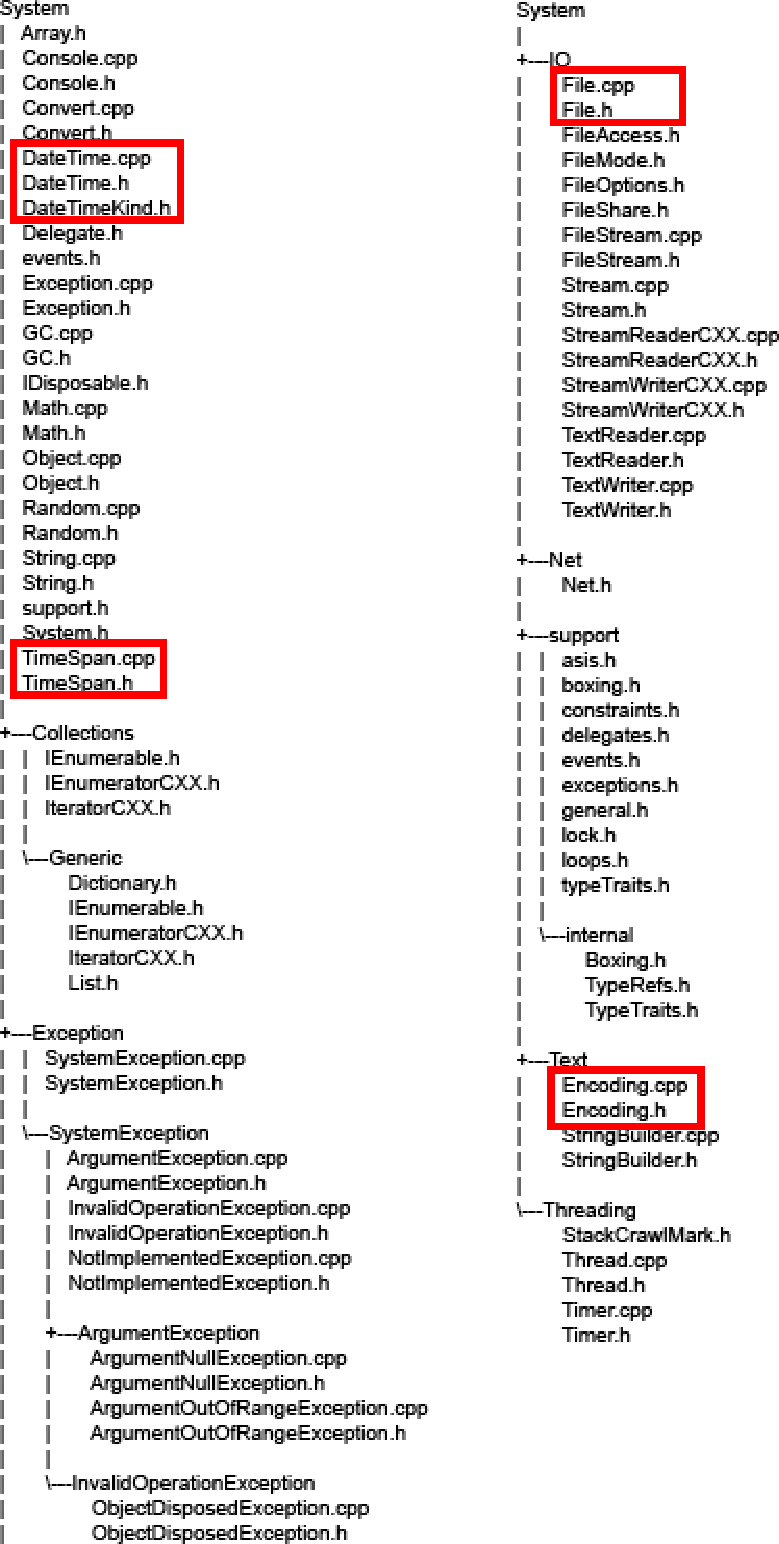
\includegraphics[width=0.75\textwidth]{pictures/appendices/alternative-cpp-classes}
  \caption{Tree dump of the C++ libraries of AlterNative currently implemented\label{fig:Libs-AlterNative}}
\end{center}\end{figure}